\documentclass[10pt]{article}
\usepackage[T1]{fontenc}
\usepackage{a4wide}
\usepackage[latin1]{inputenc}
\usepackage[english]{babel}
\usepackage{tikz}
\usetikzlibrary{calc}

\def\code#1{\texttt{#1}}
\begin{document}

\title{The \code{inflight\_rels\_buffer} structure, and underlying
concurrency considerations}

\section{Introduction}

This set of notes grew from my inline comments while decrypting the
previous \code{filter\_io.c} code, and commenting it. Beyond a 33\%
comment-to-code ratio, it seems sane to put lengthy comments aside in a
separate file.



The \code{filter\_rels} function is the main interface exported by
\code{filter\_io.c}. Its purpose is to read a large set of relation
files, and call a dedicated callback for each relation in this file. An
important requirement for this code is that callbacks must be called
\emph{in order}, according to the ordering of the relations in the input
file. The reason for this is that indices respective to the input file
set as kept later on for reference.

In this sort of process, relations undergo several different processing
steps. The most involved case is the binary filter/dup2, where relations
from new files go through the following steps:

\begin{itemize}
    \item reading raw data from the file;
    \item parsing the relation itself;
    \item converting indices to the renumber format;
    \item writing to the output file.
\end{itemize}

The crux of the story is that it is sometimes desirable to parallelize
\emph{some} of the steps.

For unessential reasons, the first step is treated separately by the
\code{ringbuf\_feed\_stream} function.

All other steps manipulate relations as their primary data object.
There's a source\footnote{The source is unique because of the strict
ordering requirement.}, which is the \code{ringbuf} type object, and one or
several sinks, which are the final output files.

The relations between the source and the sink(s) are called "in-flight".
They are stored in a special buffer called \code{inflight\_rels\_buffer}.
This buffer controls the current processing step for relations. It works
like a ring buffer of statically defined size, and holds room for
relations of type \code{earlyparsed\_relation}. The memory area for a
relation is modified in the course of its evolution through the
successive processing steps.

This memo focuses on the \code{inflight\_rels\_buffer} structure, and
describes very briefly the rest of the structures announced above, which
together form the \code{filter\_rels} function.

\section{The parsing step}

\code{filter\_rels} acts as a consumer of the data coming from the input
files. This raw data is obtained by an external thread, and
\code{filter\_rels} (itself) arranges so that it enters the sequence of
consecutive processing steps.

We therefore have the:
\begin{center}
{\fbox{
\textbf{initial pipe}: \code{filter\_rels\_producer\_thread} ---
\code{filter\_rels}}}
\end{center}


\code{filter\_rels} itself does the parsing of the relation data. Even
though only limited parsing is at stake, it represents a crucial
contention point. The main cause for this contention is the
\textbf{strict ordering requirement} which hampers faster processing.

Since parsing is limiting, \code{filter\_rels} accepts as arguments a
bitmask indicating what to parse. This in turn determines which function
will be called for parsing. Each binary is likely to be interested by
different fields in the relations, so this differs from one to another.

One this parsing step is completed, we have well-formed, somewhat-parsed
relations, of type \code{earlyparsed\_relation}, ready to start further
processing.

\section{Further processing steps: the \code{inflight\_rels\_buffer}
structure}

Relations go through different steps. A thread which "does" step $k$ is
called a "level-$k$" thread. As \code{filter\_rels} feeds relations into
the buffer, it is the (unique) level-$0$ thread.

Assuming $n$ distinct processing steps, a relation slot may be in several
states: either currently being treated, or having already been treated,
by some level $k\in [0,n[$. This makes $2n$ possible statuses.
We maintain absolute relation counts. The relation of index
\texttt{i} through the structure is at some given step if the
conditions given in table~\ref{tab:conditions} hold.

\begin{table}
\begin{center}
    \begin{tabular}{l|l|l}
state & condition & also\\
        \hline
being treated by level-$0$ & \verb|completed[0] <= i < scheduled[0]| & \\
    treated by level-$0$   & \verb|scheduled[1] <= i < completed[0]| &
        \code{level\_processed[i] >= 0}\\
being treated by level-$1$ & \verb|completed[1] <= i < scheduled[1]| & \\
    treated by level-$1$   & \verb|scheduled[2] <= i < completed[1]| &
        \code{level\_processed[i] >= 1}\\
\ldots&&\\
being treated by level-$n-1$ & \verb|completed[n-1] <= i < scheduled[n-1]| & \\
    treated by level-$n-1$   & \verb|i < completed[n-1]| & 
        \code{level\_processed[i] >= n}\\
\end{tabular}
\caption{\label{tab:conditions}Translation of the processing state of relations into \code C
relational operators}
\end{center}
\end{table}

Because of the ring buffer structure, there may be in fact only a limited
number of "in-flight" relations. Thus we also have
\verb|scheduled[0] <= completed[n-1] + SIZE_BUF_REL|. This is relatively unimportant, and is
not further discussed.

The hot spots are the moves from a step to another. We may thus consider
that we have several pipes.
\begin{center}
    \begin{itemize}
        \item \fbox{Pipe $0$: relations treated by level-$0$ --- treatment by level-$1$}
        \item \fbox{Pipe $1$: relations treated by level-$1$ --- treatment by level-$2$}
        \item \ldots
    \end{itemize}
\end{center}

The \code{inflight\_rels\_buffer} structure allows \emph{several threads}
at some given level $k$ by enforcing that a relation is always at the
same slot within the buffer.

All level-$k$ threads are thus competing for performing one of the
following operations:
\begin{itemize}
    \item \code{schedule(k)}: schedule one relation in the buffer for
        processing at level $k$, \emph{if one is available}. This has to
        possibly wait for the counted \verb|completed[k-1]| to
        increase.\\
        When a new relation has been scheduled for processing at level
        $k$, the counter \verb|scheduled[k]| is increased.
    \item \code{complete(k)}: mark a relation as having been processed at
        level $k$. If there are several level-$k$ threads, completion
        will happen in shuffled order, which needs extra care described
        below.\\
        Marking new relations as having been completed leads of
        course to increasing \verb|completed[k]|, which may thus be of
        interest to the operation \code{schedule(k+1)}.
\end{itemize}

In the terminology above, a level-$k$ thread is thus naturally between
pipes $k-1$ and $k$. The number of producers (write end) of pipe $k-1$ is
the number of level-$k-1$ threads, while its number of consumers (read
end) is the number of level-$k$ threads. A typical "vanilla"
producer-consumer pipe would be having just two single-threaded levels
indexed $0$ and $1$.

When for some $k$, there is only one level-$k$ thread, we have the
obvious identities:
\begin{itemize}
    \item \verb|scheduled[k] == completed[k] + 1| when there is
some processing going on at level $k$,
    \item \verb|scheduled[k] == completed[k]| when not.
\end{itemize}


\section{Key properties}

Concurrent accesses to the counters \verb|scheduled[k]| and
\verb|completed[k]| are protected by mutexes. For an $n$-levels buffer,
we use $n$ mutexes \verb|m[0]| to \verb|m[n-1]|.  We enforce the
following important properties during the bulk of the processing
(draining the pipe is a bit special, but not much).
\begin{itemize}
    \item \verb|scheduled[k]| is read and written \emph{only} by the
        \code{schedule(k)} call, and with {\bfseries \verb|m[k-1]| locked}.
    \item \verb|completed[k]| is accessed only with {\bfseries
        \verb|m[k]| locked}. The \code{schedule(k)} call only reads it,
        while \code{completed(k)} can update it.
\end{itemize}

For the special needs of the case with several threads doing processing
at the same level, we also have a \verb|level_processed[]| array, indexed
by the relation slot in the ring buffer. 



A \texttt{schedule(k)} call may be blocked because it so happens that
\verb|scheduled[k]==completed[k-1]|. In which case it has to wait for
\verb|completed[k-1]| to increase. This entails waiting on a condition.
We define $n$ conditions, named \verb|bored[k]|. The third key fact about
waiting is that:

\begin{itemize}
    \item Threads doing \code{schedule(k)} may wait on condition
        \verb|bored[k]|, with mutex \verb|m[k]| locked.
    \item The condition \verb|bored[k]| may be signaled by the
        \code{complete(k)} call, with mutex \verb|m[k]| locked.
\end{itemize}

Here, waiting on a condition with a mutex locked is in the sense of
\code{pthread\_cond\_wait}.


\section{Multithreading pitfalls}

The threads currently doing level-$k$ processing all operate on relations
whose index \texttt{i} in the ring buffer is such that
\verb|completed[k]<=i<scheduled[k]|. In case level-$k$ is multithreaded,
we have no ordering guarantee on the completion order of these calls.

Here we describe a behaviour which uses the pthreads mechanisms for
serialization. Discussions regarding lightweight busy waits come later.

Upon completion, a thread acquires the mutex \verb|m[k]|. It may thus
update \verb|completed[k]|. In order to do so, it must observe whether it
can, in the first place: it might be that other relation slots are still
undergoing some processing, maybe some which have been scheduled quite
earlier than the current thread. Let $i_0$ denote the relation index
being processed by the current thread. The procedure is as follows:
\begin{itemize}
    \item Acquire \verb|m[k]|.
    \item Start reading \verb|level_processed[i]| for
        \verb|i=completed[k]| onwards. \textbf{Stop at $i=i_0$}.
    \item Set \verb|completed[k]| to the largest index $i$ looked for which
        \verb|level_processed[i]==k|, and to $i+1$ if $i=i_0$.
    \item Increment \verb|level_processed[i0]| to $k$.
    \item Signal \verb|bored[k]| to awake all waiters.
    \item Release \verb|m[k]|.
\end{itemize}

It is important to avoid the temptation of detecting finished threads for
indices \emph{above} $i_0$. This is because while we know that
\verb|scheduled[k]>=i0|, we do not have the freedom to \emph{read} the
counter \verb|scheduled[k]| in a safe manner.


The downside of this approach is that if that there is potential for
\verb|completed[k]| to be updated with some delay. If two threads,
numbered $0$ and $1$, process relation slots $0$ and $1$, and if thread
$0$ completed \emph{after} thread $1$, then \verb|completed[k]| will be
updated to $1$ upon completion of thread $0$, while at this point
relation $1$ is also processed. In order for \verb|completed[k]| to catch
up, we rely on further processing to update it as a side effect.

A graphical representation of a typical state of the in-flight buffer
is given by Figure~\ref{tab:levelprocessed}.


This has consequences regarding how draining must be achieved.


\begin{figure}
    \begin{center}
\makeatletter
  \def\mark#1{\@ifnextchar[{\marki#1}{\marki#1[]}}
  \def\marki#1[#2]#3;{\draw (7.2*#1:2.5cm) 
  edge[<-] (7.2*#1:3.0cm) (7.2*#1:3.1cm) node[#2]{#3};}
  \def\paint#1#2#3{%
      \draw[line width=5mm,#3](0,0) + (#1*7.2:2.25) arc
      (#1*7.2:#2*7.2:2.25cm);
  }
  \def\markcell#1#2#3{%
      \paint{#1}{(#1+1)}{#3}
      \node at (#1*7.2+3.6:2.25cm) {\sffamily\tiny #2};
  }
  \def\completed#1#2;{\markcell{#2}{#1}{completed#1}}
  \def\scheduled#1#2;{\@tempcnta=#1\advance\@tempcnta-1\relax\edef\less{\the\@tempcnta}\markcell{#2}{\less}{scheduled#1}}

\makeatother
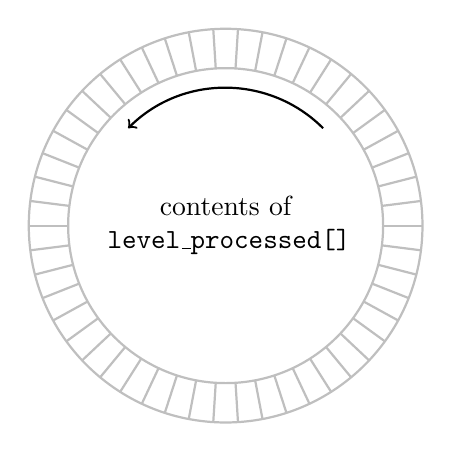
\begin{tikzpicture}[thick,
        scheduled0/.style={red!20!white},
        scheduled1/.style={green!20!white},
        scheduled2/.style={blue!20!white},
        completed0/.style={red!50!white},
        completed1/.style={green!50!white},
        completed2/.style={blue!50!white}
]
    \foreach \d in {7.2,14.4,...,360} \draw[lightgray] (\d:2cm)--(\d:2.5cm);
    \draw[lightgray](0,0) circle (2cm) (0,0) circle (2.5cm);
    \node(0,0) {\parbox{3cm}{\centering contents of
    \code{level\_processed[]}}};
    \draw[->](0,0) + (45:1.75) arc (45:135:1.75);
\mark{0}{0};
    \completed2 0;
    \completed2 1;
    \completed2 2;
    \completed2 3;
    \completed2 4;
    \completed2 5;
\mark{6}[anchor=west]{\code{completed[2]}};
    \scheduled2 6;
    \completed2 7;
    \completed2 8;
    \scheduled2 9;
\mark{10}[anchor=south west]{\code{scheduled[2]}};
    \completed1 10;
    \completed1 11;
    \completed1 12;
    \completed1 13;
    \completed1 14;
    \completed1 15;
\mark{16}[anchor=south east]{\code{completed[1]}};
    \scheduled1 16;
    \completed1 17;
    \scheduled1 18;
    \scheduled1 19;
    \completed1 20;
    \completed1 21;
\mark{22}[anchor=east]{\code{scheduled[1]}};
    \completed0 22;
    \completed0 23;
    \completed0 24;
    \completed0 25;
    \completed0 26;
    \completed0 27;
    \completed0 28;
    \completed0 29;
    \completed0 30;
\mark{31}[anchor=north east]{\code{completed[0]}};
    \scheduled0 31;
\mark{32}[anchor=north]{\code{scheduled[0]}};
  % \draw(0,0) +(331.2:2.5cm) node[anchor=north west] {"`bad"': 8 (16\%)};
  % \draw(0,0) +(266.4:2.8cm) node[anchor=north] {"`ok"': 10 (20\%)};
  % \draw(0,0) +(198:2.8cm) node[anchor=north east] {"`good"': 9 (18\%)};
  % \draw(0,0) +(154.8:2.8cm) node[anchor=south east] {"`very good"': 3 (6\%)};
  % \draw(0,0) +(72:2.8cm) node[anchor=south] {"`none"': 20 (40\%)};
\end{tikzpicture}
\caption{\label{tab:levelprocessed}Graphical representation of the
current status of \texttt{level\_processed[]}.}
    \end{center}
\end{figure}

\section{Use of lightweight locking}

We consider here a memory model where a memory read to a location currently
being updated may return only either the old, or the new value. This is
the case of most typical computers. Here, it is possible to avoid the
serialization layer of the POSIX threads, and use "simple busy waits", as
follows:
\begin{itemize}
    \item acquire/release a lock: do nothing.
    \item wait on a condition: do a very small sleep, and actually check
        the condition.
    \item signal a condition: do nothing.
\end{itemize}

This may work only in the case where we have structural guarantee that
\emph{only one thread} may write to a given variable at a given time.

For our $n$-level buffer, this can work if we have no multithreading at
the different levels. This uses the same code, the locking infrastructure
being passed as a template parameter to the code. The critical
\code{schedule(k)} and \code{complete(k)} are specialized for this case.
\end{document}
